\documentclass[11pt]{article}
\usepackage{tikz}

\usetikzlibrary{arrows}

\begin{document}

\section*{FSM for Server}
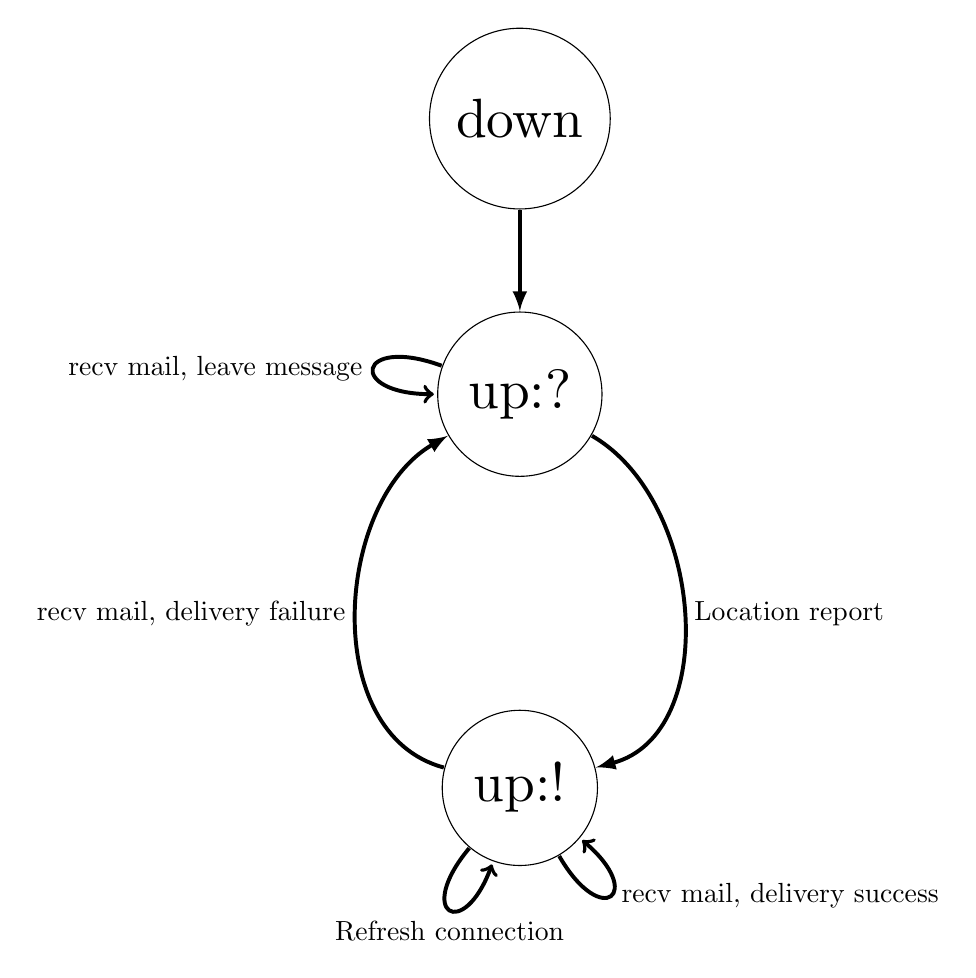
\begin{tikzpicture}
\node[draw, circle, scale=2] at (0,8.5) (down) {down};
\node[draw, circle, scale=2] at (0,5) (upUk) {up:?};
\node[draw, circle, scale=2] at (0,0) (upK) {up:!};

\draw[arrows={-latex}, line width=.5mm, scale=2] (down) to (upUk);
%location unknown to known
\draw[arrows={-latex}, line width=.5mm, scale=2]
  (upUk) to [out=330, in=15] node[right] {Location report} (upK);
%known -> unknown
\draw[arrows={-latex}, line width=.5mm, scale=2]
  (upK) to [out=165, in=210] node[left] {recv mail, delivery failure} (upUk);

\path[arrows={-latex}, out=230, in=250, distance=30mm, line width=.5mm]
  (upK) edge[loop] node[below] {Refresh connection} (upK);
\path[arrows={-latex}, out=300, in=320, distance=30mm, line width=.5mm]
  (upK) edge[loop] node[right] {recv mail, delivery success} (upK);

\path[arrows={-latex}, out=160, in=180, distance=30mm, line width=.5mm]
  (upUk) edge[loop] node[left] {recv mail, leave message} (upUk);

\end{tikzpicture}

\subsection*{States}
\begin{itemize}
\item down \\
The service on the Server is not running.
\item up:? \\
The Server is running, but the message channel is down. A `?' means the routing
address of the Receiver is not known.
\item up:! \\
The Server is running and it has establish a message channel with the Receiver.
\end{itemize}

\subsection*{Recv mail, leave message}
The Sender sends mail to the Server but the message channel is down. The server
saves the message and delivers it when the message channel is next established.
\subsection*{Recv mail, delivery failure}
The Sender sends mail to the Server. The Server attempts to deliver it to the
Receiver, but the message channel was stale(i.e. the Receiver moved). The
Server saves the message and delivers it when the message channel is next
established.
\subsection*{Refresh connection}
The Server sends a refresh message over the message channel to keep the
connection open. This is for NAT traversal to prevent the initial connection
from being killed.
\subsection*{Recv mail, delivery success}
The Sender sends mail to the Server. The Server successfully delivers it to the
Receiver and the message channel remains established.
\subsection*{Location report}
The Receiver transitions from down to up and the message channel is
established.

\pagebreak

\section*{FSM for Receiver}
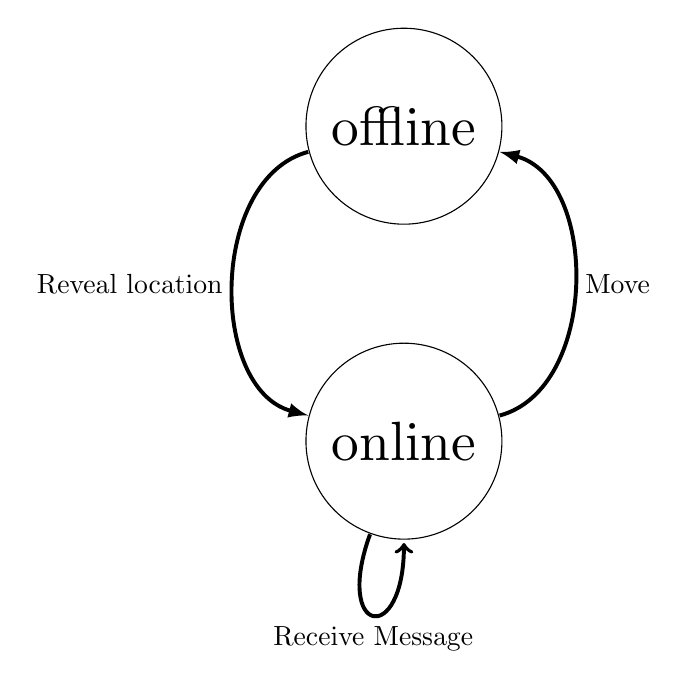
\begin{tikzpicture}
\node[draw, circle, scale=2] at (0,4) (off) {offline};
\node[draw, circle, scale=2] at (0,0) (on) {online};
\draw[arrows={-latex}, line width=.5mm, scale=2] (off) to [out=195, in=165]
  node[left] {Reveal location} (on);
%self edge
\path[arrows={-latex}, out=250, in=270, distance=30mm, line width=.5mm]
  (on) edge[loop] node[below] {Receive Message} (on);
\draw[arrows={-latex}, line width=.5mm, scale=2] (on) to [out=15, in=-15]
  node[right] {Move} (off);
\end{tikzpicture}

\subsection*{Reveal location}
The Receiver makes an initial connection to Server, bootstraping the message
channel.
\subsection*{Receive Message}
The Server sends a message to the Receiver via the message channel and authenticates
it.
\subsection*{Move}
The Receiver moves, connecting to a different network or otherwise not
listening on the message channel.


\end{document}
